\documentclass[class=report, crop=false, 12pt,a4paper]{standalone}
\usepackage{enumitem}
\usepackage{multicol}
\usepackage{graphicx}
\usepackage{float}
\usepackage{amsmath}
\usepackage{amssymb}
\usepackage{mathtools}
\usepackage{siunitx}
\usepackage{commath}
\usepackage{array}
\usepackage{natbib}
\usepackage{cancel}
\usepackage[a4paper,width=150mm,top=25mm,bottom=25mm]{geometry}
\setlength{\parindent}{0pt}
\begin{document}
\section{Thick wall cylinders}
Lame's equations
\begin{align}
    \sigma_r &= \frac{p_i r_i^2 - p_or_o^2}{r_o^2 - r_i^2} - \frac{\left(p_i-p_o\right)r_i^2 r_o^2}{\left(r_o^2 - r_i^2\right)r^2}\\
    \sigma_{\theta} &= \frac{p_i r_i^2 - p_o r_o^2}{r_o^2 r_i^2} + \frac{\left(p_i-p_o\right)r_i^2 r_o^2}{\left(r_o^2 - r_i^2\right)r^2}
\end{align}
We have seen that a thick cylinder subjected to internal pressure experiences very high peaks of stress at the inner surface. 
\begin{figure}[H]
    \centering
    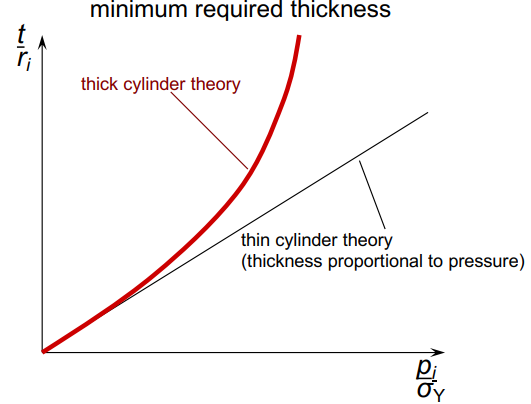
\includegraphics[height = 5cm]{../img/diagram118.png}
    \caption{The required thickness increases non-linearly with the pressure.}
\end{figure}
The design of cylinders that have to maintain high levels of pressure requires specific strategies. aimed at reducing the hoop stress levels at the inside surface.
\begin{figure}[H]
    \centering
    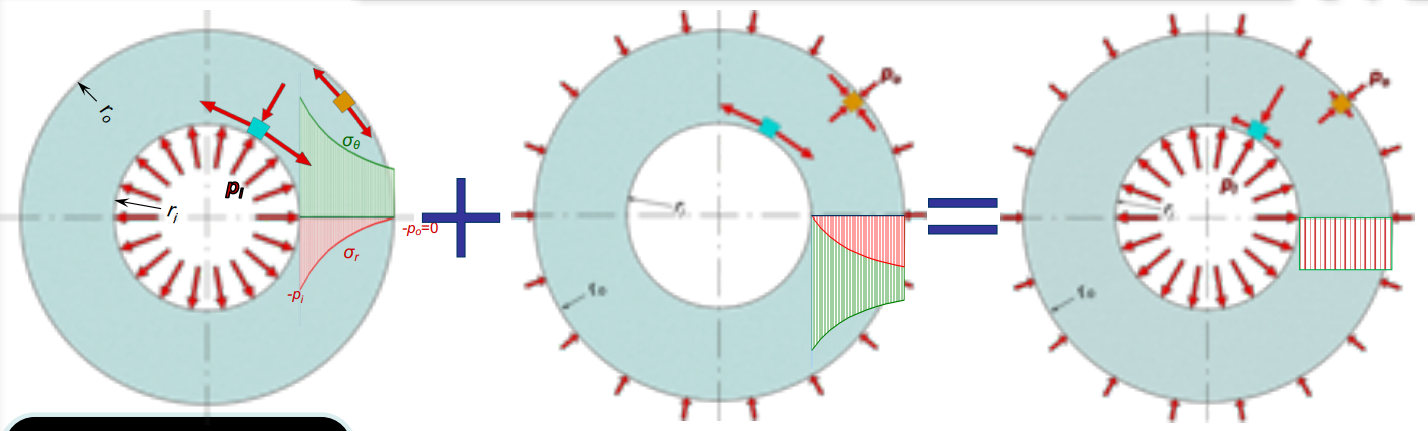
\includegraphics[width = \textwidth]{../img/diagram119.png}
    \caption{}
\end{figure}
A possible solution could be reducing the level of hoop stress by increasing the pressure at the outer surface.
\section{Compound cylinders}
\subsection{Containing high pressures}
This can be done by shrinking another tube on the outside of the original one:
\begin{figure}[H]
    \centering
    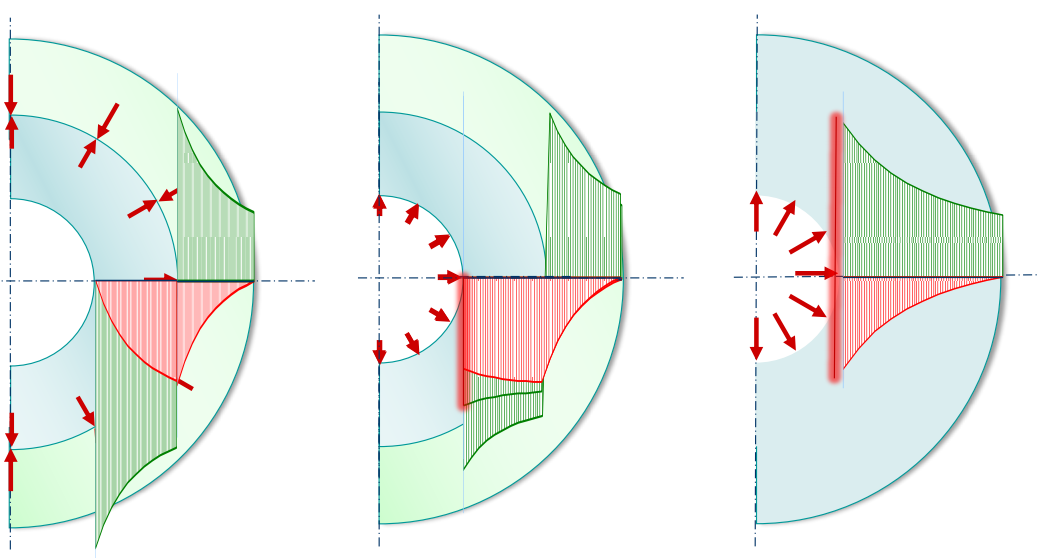
\includegraphics[width = \textwidth]{../img/diagram120.png}
    \caption{}
\end{figure}
\subsection{Compound or 'built-up' cylinders}
THis compound (or built-up) arrangement is obtained by assembling two cylinders with initial diametrical interference $\delta$ at room temperature. The outer cylinder is heated and the inner cylinder is cooled, in order to compensate for the interference by thermal expansion/contraction and allow assembly. Returning the components to room temperature, a set of residual radial and hoop stress is introduced, which locks the two components firmly together. 

The interference between the two cylinders will produce an external pressure $p_{int}$ acting on the internal cylinder, and an equal internal pressure $p_{int}$ acting on the external cylinder, function of the interference $\delta$. 
\begin{figure}[H]
    \centering
    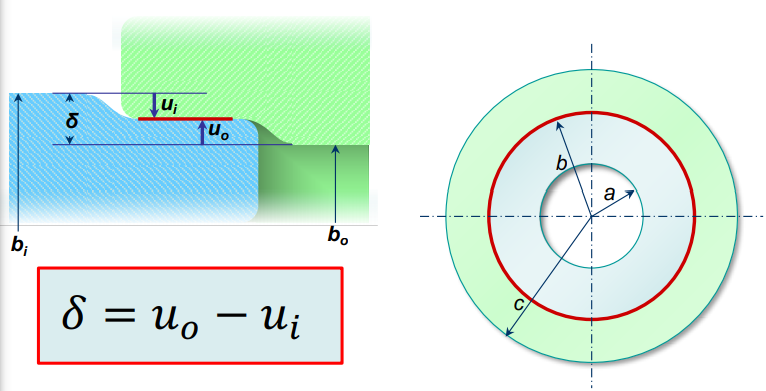
\includegraphics[height = 5cm]{../img/diagram121.png}
    \caption{}
\end{figure}
Interface pressure can be expressed as a function of the interference, by using the solid mechanics equations.
\subsubsection{Other applications}
\begin{figure}[H]
    \centering
    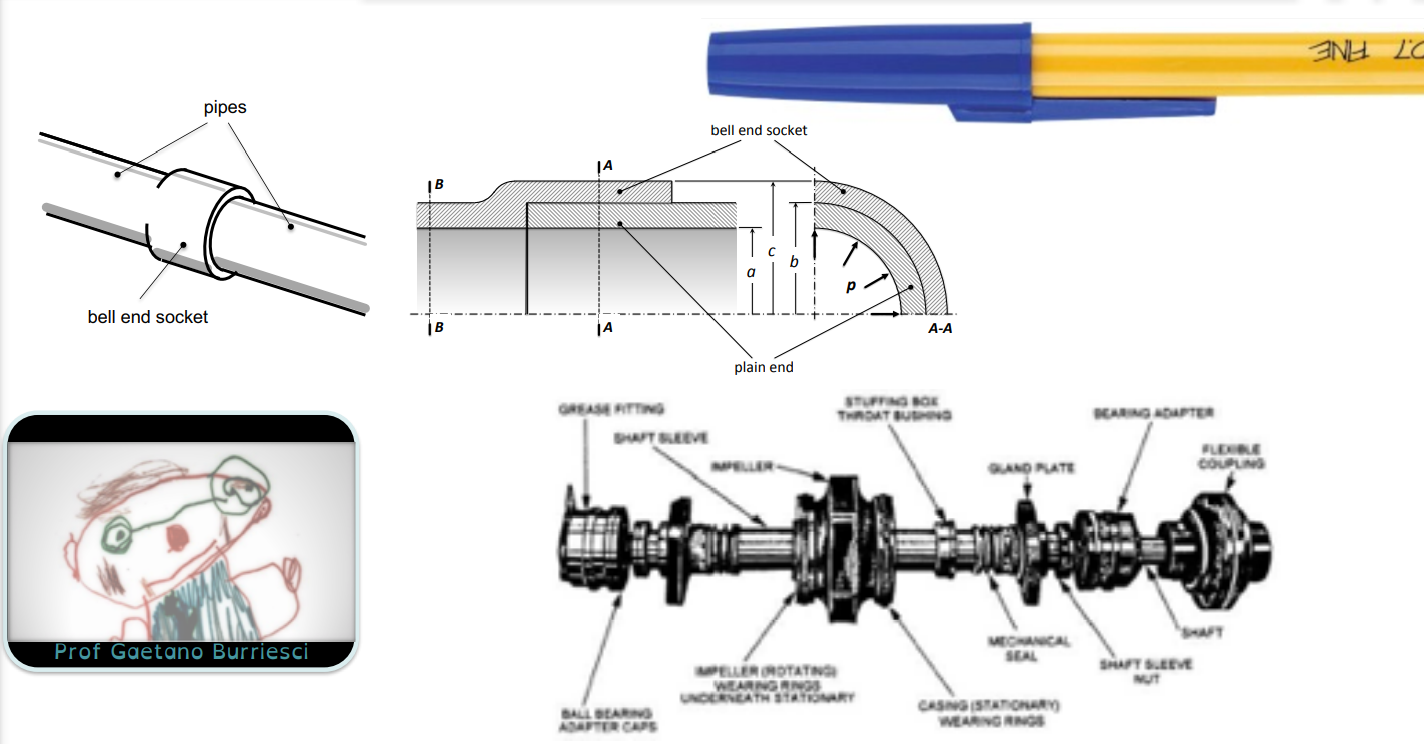
\includegraphics[width = \textwidth]{../img/diagram122.png}
    \caption{}
\end{figure}
\subsection{Stress state at the interface}
\begin{figure}[H]
    \centering
    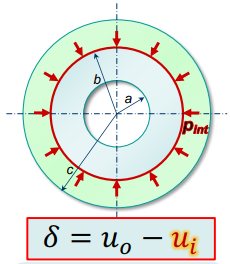
\includegraphics[height = 5cm]{../img/diagram123.png}
    \caption{}
\end{figure}
\begin{gather}
    u = \frac{r}{E}\left(\sigma_{\theta} - v \sigma_r\right)\\
    \rightarrow u_i = \frac{b}{E_i}\left[\sigma_{\theta, i} \left(b\right) - v_i \sigma_{r,i} (b)\right]
\end{gather}
Lame's equations:
\begin{gather}
    \sigma_r = A - \frac{B}{r^2}\\
    \sigma_{\theta} = A + \frac{B}{r^2}
\end{gather}
Boundary conditions:
\begin{gather}
    \sigma_{r,i}(a) = 0 = A - \frac{B}{a^2}\\
    \sigma_{r,i}(b) - -p_{int} = A - \frac{B}{b^2}\\
    A = -p_{int}\frac{b^2}{b^2 - a^2}\\
    B = -p_{int}\frac{a^2 \cdot b^2}{b^2 - a^2}
\end{gather}
Substituting:
\begin{equation}
    \sigma_{\theta,i} = A + \frac{B}{r^2} = -p_{int}\frac{b^2}{B^2 - a^2} \left(1 + \frac{a^2}{r^2}\right)
\end{equation}
Therefore:
\begin{gather}
    \sigma_{r,i}(b) = -p_{int} \hspace{1cm} \sigma_{\theta,i}(b) = -p_{int}\frac{b^2 + a^2}{b^2 - a^2}\\
    u_i = -p_{int} \frac{b}{E_i} \left(\frac{b^2 + a^2}{b^2 - a^2} - v_i\right)
\end{gather}
\begin{figure}[H]
    \centering
    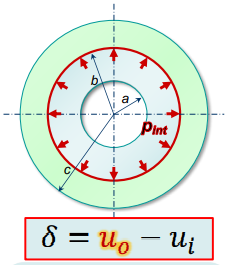
\includegraphics[height = 5cm]{../img/diagram124.png}
    \caption{}
\end{figure}
\begin{gather}
    u_o = \frac{b}{E_o}\left[\sigma_{\theta,o} (b) - v_o \sigma_{r,o}(b)\right]
\end{gather}
Lame's equations:
\begin{gather}
    \sigma_r = A - \frac{B}{r^2}\\
    \sigma_{\theta} = A + \frac{B}{r^2}
\end{gather}
Boundary conditions:
\begin{gather}
    \sigma_{r,o}(b) = -p_{int} = A - \frac{B}{b^2}\\
    \sigma_{r,o}(c) = 0 = A - \frac{B}{c^2}\\
    A = -p_{int} \frac{b^2}{b^2- c^2}\\
    B = -p_{int} \frac{b^2 \cdot c^2}{c^2 - b^2}
\end{gather}
Substituting:
\begin{gather}
    \sigma_{\theta,o} = A + \frac{B}{r^2} = -p_{int} \frac{b^2}{c^2 - b^2} \left(1+ \frac{c^2}{r^2}\right)
\end{gather}
Therefore:
\begin{gather}
    \sigma_{r,o}(c) = 0 \hspace{1cm} \sigma_{\theta,o}(b) = p_{int}\frac{c^2 + b^2}{c^2 -b^2}\\
    u_o = p_{int} \frac{b}{E_o}\left(\frac{c^2 + b^2}{c^2 - b^2} + v_o\right)
\end{gather}
\subsection{Analysis of compound cylinders}
\begin{figure}[H]
    \centering
    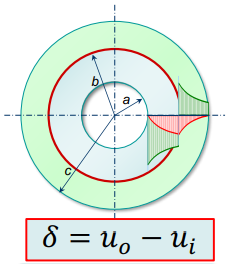
\includegraphics[height = 5cm]{../img/diagram125.png}
    \caption{}
\end{figure}
\begin{gather}
    u_i =-p_{int}\frac{b}{E_i}\left(\frac{b^2 + a^2 }{b^2 - a^2}-v_i\right)\\
    u_o = p_{int}\frac{b}{E_o}\left(\frac{c^2 + b^2 }{c^2 - b^2}+v_o\right)\\
    \delta = p_{int}b\left[\frac{1}{E_o}\left(\frac{c^2 + b^2}{c^2 - b^2}+v_o\right) + \frac{1}{E_i}\left(\frac{b^2 + a^2}{b^2 - a^2}-v_i\right)\right]
\end{gather}
For a single material: $E_i = E_o = E$, and $v_i = v_o = v$:
\begin{gather}
    \delta = p_{int} \frac{b}{E}\left[\frac{2b^2\left(c^2-a^2\right)}{\left(c^2 - b^2\right)\left(b^2-a^2\right)}\right]\\
    p_{int} = E \delta \left[\frac{\left(c^2 + b^2\right)\left(b^2 - c^2\right)}{2b^3\left(c^2 - a^2\right)}\right]
\end{gather}
One $p_{int}$ is known, it can be used in the Lame's expressions, to determine the stress state in the two cylinders. 
\begin{figure}[H]
    \centering
    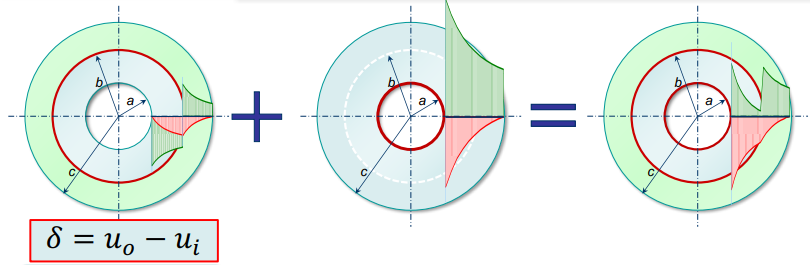
\includegraphics[width = \textwidth]{../img/diagram126.png}
    \caption{}
\end{figure}
In the case of internal pressure, under linear elastic conditions, the stress distribution can be obtained by selecting suitable BCs, or by superposition with the distribution of a single cylinder of equivalent wall thickness subjected to the internal pressure.
\section{Rotating discs}
\begin{figure}[H]
    \centering
    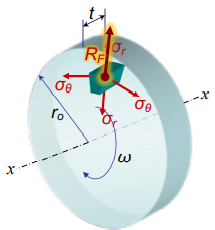
\includegraphics[height = 5cm]{../img/diagram127.png}
    \caption{}
\end{figure}
Consider a circular disc of outer radius $r_{o}$, rotating about an axis of symmetry with constant angular velocity $\omega$. Centripetal acceleration can produce high stresses that may compromise the disc integrity. If the disc is thin, longitudinal stresses can be neglected and the state of stress is plane. Under these conditions the same approach used for thick cylinders can be used.
\subsection{Solid mechanics equations}
\subsubsection{Equilibrium equations}
\begin{figure}[H]
    \centering
    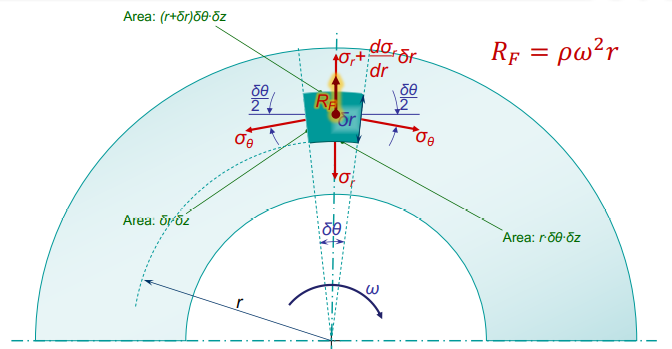
\includegraphics[height = 6cm]{../img/diagram129.png}
    \caption{}
\end{figure}
For thick cylinders: 
\begin{equation}
    \frac{\dif \theta_r}{\dif r} + \frac{\sigma_r - \sigma_{\theta}}{r} =0 
\end{equation}
Radial equilibrium:
\begin{equation}
    \frac{\dif \theta_r}{\dif r} + \frac{\sigma_r - \sigma_{\theta}}{r} + \rho \omega^2 r = 0
\end{equation}
\subsubsection{Compatbility relations}
\begin{figure}[H]
    \centering
    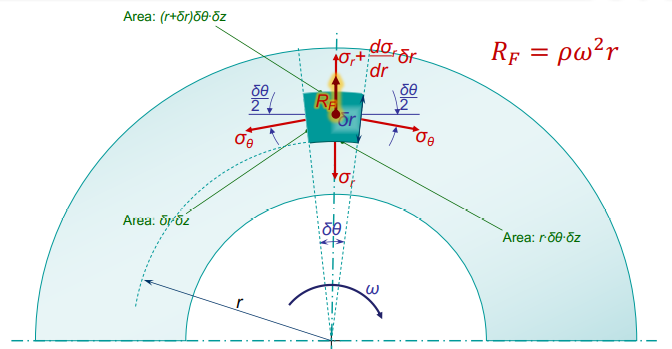
\includegraphics[height = 6cm]{../img/diagram129.png}
    \caption{}
\end{figure}
Same as in thick cylinders:
\begin{gather}
    \varepsilon_r = \frac{\dif u}{\dif r}\\
    \varepsilon_{\theta} = \frac{u}{r}
\end{gather}
\subsubsection{Constitutive laws}
Plane stress state:
\begin{gather}
    \sigma_r = \frac{E}{1-v^2} \left(\varepsilon_r + v \varepsilon_{\theta}\right)\\
    \sigma_{\theta} = \frac{E}{1-v^2} \left(\varepsilon_{\theta} + v \varepsilon_{r}\right)
\end{gather}
\subsection{Differential equation}
Combining all of our solid mechanics equations we can form an Euler's differential equation.
\begin{gather}
    u''r^2 + u'r -u=-\frac{1-v^2}{E}\rho\omega^2 r^3
\end{gather}
Complementary function (same as for thick cylinders):
\begin{gather}
    u_{CF} = Ar + \frac{B}{r}
\end{gather}
Particular integral, general form:
\begin{gather}
    u = Ar^3 + Br^2 + Cr + D\\
    u' = 3Ar^2 + 2Br + C\\
    u'' = 6Ar + 2B
\end{gather}
Substituting:
\begin{gather}
    6Ar^3 + 2Br^2 + 3Ar^3 + 2Br^2 + Cr - Ar^3 - Br^2 - Cr - D = - \frac{1-v^2}{E} \rho \omega^2 r^3\\
    8 Ar^3 + 4Br^2 - D = - \frac{1-v^2}{E}\rho\omega^2 r^3
\end{gather}
Comparing these terms:
\begin{gather}
    B = C = D = 0; \, A = -\frac{1-v^2}{8E}\rho\omega^2\\
    u_{PI} = - \frac{1-v^2}{8E}\rho\omega^2 r^3
\end{gather}
General solution:
\begin{gather}
    u = Ar + \frac{B}{r} - \frac{1-v^2}{E} \frac{\rho\omega^2 r^3}{8}
\end{gather}
\subsection{Axisymmetric stresses}
Differentiating:
\begin{gather}
    u = Ar + \frac{B}{r} - \frac{1-v^2}{E} \frac{\rho\omega^2 r^3}{8}\\
    u' = A - \frac{B}{r^2} \frac{1-v^2}{E}\frac{\rho \omega^2 r^3}{8}
\end{gather}
Substituting into constitutive laws:
\begin{gather}
    \sigma_r = C - \frac{D}{r^2} - \frac{3 + v}{8}\rho \omega^2 r^2\\
    \sigma_{\theta} = C + \frac{D}{r^2} - \frac{1+ 3v}{8}\rho\omega^2 r^2 
\end{gather}
\subsection{Continuous discs}
\begin{figure}[H]
    \centering
    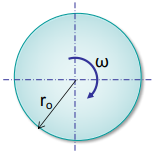
\includegraphics[height = 5cm]{../img/diagram130.png}
    \caption{}
\end{figure}
\begin{gather}
    \sigma_r = C - \frac{D}{r^2} - \frac{3 + v}{8}\rho \omega^2 r^2\\
    \sigma_{\theta} = C + \frac{D}{r^2} - \frac{1+ 3v}{8}\rho\omega^2 r^2 
\end{gather}
Boundary conditions:
\begin{gather}
    \sigma_r (0) \neq \infty \; \& \; \sigma_{\theta} (0) \neq \infty \rightarrow D = 0 \rightarrow \sigma_r = C - \frac{3+v}{8} \rho \omega^2 r^2\\
    \sigma_r \left(r_0\right) = 0 \rightarrow C - \frac{3+v}{8} \rho \omega^2 r^2_o = 0 \rightarrow C = \frac{3+v}{8}\rho \omega^2 r^2_o
\end{gather}
Substituting:
\begin{gather}
    \sigma_r = \frac{3+v}{8} \rho \omega^2 \left(r_o^2 - r^2\right)\\
    \sigma_{\theta} = \frac{3+v}{8}\rho \omega^2 r_o^2 - \frac{1+3v}{8} \rho \omega^2 r^2
\end{gather}
\begin{figure}[H]
    \centering
    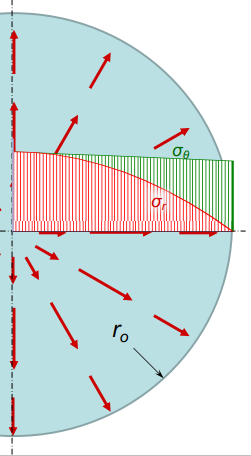
\includegraphics[height = 5cm]{../img/diagram131.png}
    \caption{}
\end{figure}
Max stress at the centre of the disc $(r=0)$:
\begin{equation}
    \sigma_{MAX} = \sigma_r (0) = \sigma_{\theta} (0) = \frac{3+v}{8}\rho \omega^2 r^2_o
\end{equation}
\begin{figure}[H]
    \centering
    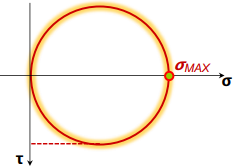
\includegraphics[height = 5cm]{../img/diagram132.png}
    \caption{}
\end{figure}
\subsection{Discs with central hole}
\begin{figure}[H]
    \centering
    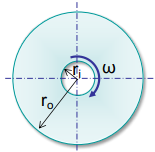
\includegraphics[height = 5cm]{../img/diagram133.png}
    \caption{}
\end{figure}
\begin{gather}
    \sigma_r = C - \frac{D}{r^2} - \frac{3 + v}{8}\rho \omega^2 r^2\\
    \sigma_{\theta} = C + \frac{D}{r^2} - \frac{1+ 3v}{8}\rho\omega^2 r^2 
\end{gather}
Boundary conditions:
\begin{gather}
    \sigma_r \left(r_i\right) = 0 \rightarrow C - \frac{D}{r_i^2} - \frac{3+v}{8} \rho \omega^2 r_i^2 = 0 \rightarrow C = \frac{3+v}{8} \rho \omega^2 \left(r_i^2 + r_o^2\right)\\
    \sigma_r \left(r_o\right) = 0 \rightarrow C - \frac{D}{r_o^2} - \frac{3+v}{8} \rho \omega^2 r_o^2 = 0 \rightarrow D = \frac{3+v}{8} \rho \omega^2 r_i^2 r_o^2 
\end{gather}
Substituting:
\begin{gather}
    \sigma_r = \frac{3+v}{8} \rho \omega^2 \left(r_i^2 + r_o^2 - \frac{r_i^2 r_o^2}{r^2}-r^2\right)\\
    \sigma_{\theta} = \frac{3+v}{8}\rho \omega^2 \left(r_i^2 + r_o^2 + \frac{r_i^2 r_o^2}{r^2} - \frac{1+3v}{3+v}r^2 \right)
\end{gather}
\begin{figure}[H]
    \centering
    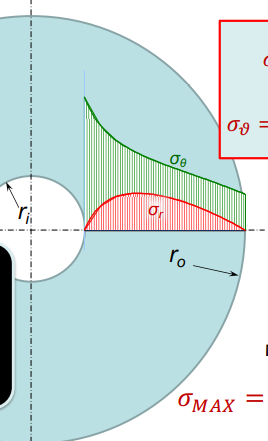
\includegraphics[height = 5cm]{../img/diagram134.png}
    \caption{}
\end{figure}
Max stress at inner radius $\left(r = r_i\right)$:
\begin{equation}
    \sigma_{MAX} = \sigma_{\theta} \left(r_i\right) = \frac{\rho \omega^2 }{4}\left[\left(3+v\right) r_o^2 + \left(1-v\right)r_i^2\right]
\end{equation}
\begin{figure}[H]
    \centering
    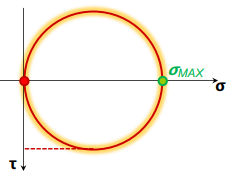
\includegraphics[height = 5cm]{../img/diagram135.png}
    \caption{}
\end{figure}
\end{document}